\subsection{Interfaz de la sección ``Mis campañas''}
En la parte izquierda de la página web, el usuario podrá ver una barra de navegación que contiene un ícono de un tractor. Al dar clic en este tractor, el usuario será dirigido a la sección ``Mis campañas''.

En esta sección también se utiliza el componente ``Skeleton'' para indicar que se está cargando la información.

Cuando se cargan la información, el Frontend recibe todas las campañas activas y las campañas en las que se encuentra inscrito el usuario. Antes de construir la interfaz, se realiza un filtrado de los resultados obtenidos. Dentro del arreglo que contiene las campañas activas se buscan coincidencias con el arreglo que contiene las campañas en las que está inscrito el usuario; las campañas que se encuentren en ambos arreglos se almacenan en un nuevo arreglo, y las que no coincidan se ignoran.

Este nuevo arreglo es el que se utiliza para renderizar las Cards de las campañas, y de esta manera sólo se le muestran al usuario sus campañas correspondientes (Ver Figura 8).

    \begin{figure}[H]
        \begin{center}
            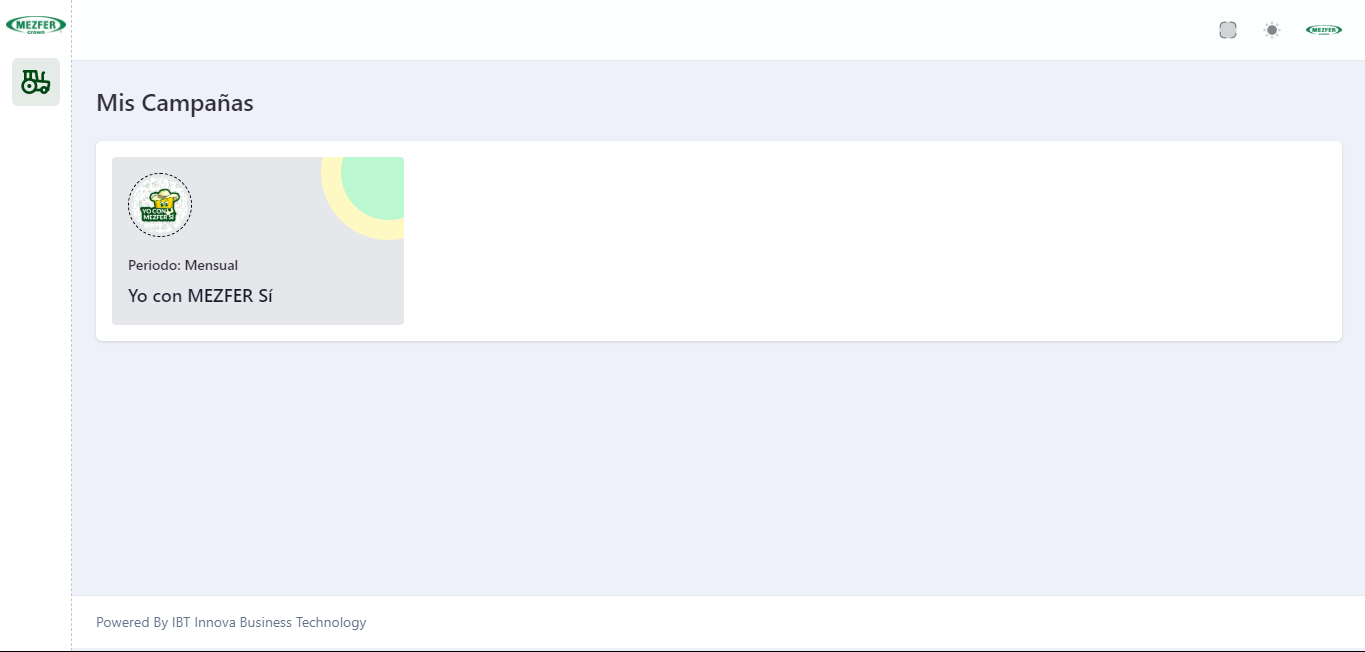
\includegraphics[scale=0.35]{img/actividades/campanias/mis-campanias.png}
            \caption{Sección ``Mis campañas''.}
            \label{fig:seccion-campañas}
        \end{center}
    \end{figure}